% \todo{We take an energy perspective on mle and manifest how to translate this formulation into Transformer architecture by leveraging Hopfield function to quantize these two terms}
% \todo{how to bring in the definition of Emch}
In this section, we translate the proposed instantiation into two modified Hopfield energy functions defined on hyperspheres (see Appendix~\ref{section:preliminaries} for preliminaries and definition of Hopfield energy $E_\text{MCH}$ in~\Eqref{eq:mch}). Through iterative energy minimization, the architectural components of Transformer layers naturally arise under this framework. The overview is presented in Figure~\ref{fig:overview}.   

% \vspace{-0.5cm}
\subsection{Hyperspherical Energy}
\label{section:hyperspherical energy}
\begin{figure*}[tbp]
    \centering
    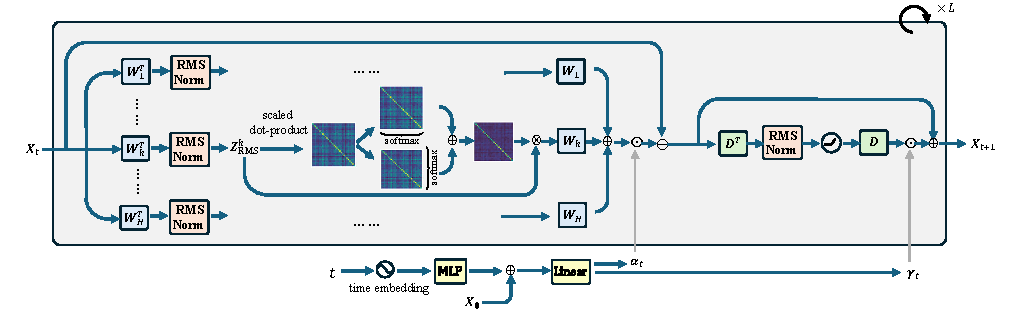
\includegraphics[width=\textwidth]{figures/overviewofHyperSET_v1.pdf}
    % \vskip -0.1in
    \caption{Overview of hyperspherical energy Transformer layer. It recovers sequential stacking of symmetric self-attention, feedforward, skip connection, and $\operatorname{RMSNorm}$ from sheer minimization of extended Hopfield energy. Adaptive step sizes are learned given the current $t$ and initial input $\mX_0$.}
    % \vskip -.2in
    \label{fig:overview}
\end{figure*}
% We consider $N$ vectors $\mX = [\vx_1, \dots, \vx_N]$ from a probabilistic space with $\vx_i \in \mathbb{R}^d, i\in [N]$, which can be seen as the contextual tokens in Transformers, and denote two different sets of basis vectors of this $d$-dimensional space, $\mW = [\mW_1, \dots, \mW_H] \in \mathbb{R}^{d\times Hp}$ and $\mD = [\vd_1, \dots, \vd_M] \in \mathbb{R}^{d\times M}$. Here, $\mW_i \in \mathbb{R}^{d\times p}$ represents the projection to the $p$-dimensional subspace. Unless otherwise specified, we assume the column vectors are incoherent and span the full space, i.e., $Hp=M=d$.
Let $\mX = [\vx_1, \dots, \vx_N]$ denote a set of $N$ contextual token vectors, each $\vx_i \in \mathbb{R}^d$. These tokens are projected into $H$ distinct subspaces via basis matrices $\mW = [\mW_1, \dots, \mW_H] \in \mathbb{R}^{d \times Hp}$, where each $\mW_h \in \mathbb{R}^{d \times p}$ spans a $p$-dimensional subspace. Additionally, we define a second set of bases $\mD = [\vd_1, \dots, \vd_M] \in \mathbb{R}^{d \times M}$ to encode semantic directions in the original space. Unless otherwise specified, we assume these basis vectors are incoherent and span the full space, \ie, $Hp = M = d$.

\subsubsection{Overcoming Token Synchronization via Repulsive Dynamics}
% A recent study \citep{yu2023white} argues that the contextual tokens lie on a low-dimensional manifold of their high-dimensional ambient space. We adopt this view and study the projection of tokens with bases $\mW$; for a subspace spanned $\mW_h$, the latent representation of token $\vx_i$ can be written as: 
Motivated by a recent argument that the contextual tokens lie on a low-dimensional manifold of their high-dimensional ambient space \citep{yu2023white}, we study the projection of tokens with bases $\mW$; for a subspace spanned by $\mW_h$, the latent representation of a token $\vx_i$ can be written as 
\begin{equation}
\label{eq:1}
    \vz_i^h = \mW_h^\top\vx_i.
\end{equation}
% \todo{refer to appendix for definition}
Canonical Hopfield energy $E_\text{MCH}$ tends to align vectors with stored patterns. This interaction often occurs between dynamic tokens and static patterns. However, in Transformers' self-attention, this interplay happens among all dynamic tokens simultaneously. Enforcing strict alignment among them risks collapsing representations into degenerate clusters, reducing expressiveness. This phenomenon has been observed empirically as oversmoothing \citep{chen2022principle,wu2024demystifying} or rank collapse \citep{pmlr-v139-dong21a}, and theoretically characterized in \citep{geshkovski2023the}. It also relates to the synchronization effect in coupled systems \citep{acebron2005kuramoto,miyato2025artificial}. 

Therefore, to overcome this issue, we extend the Hopfield energy $E_\text{MCH}$ to model the repulsive force among tokens and quantify their distributional uniformity in each subspace, which serves as a surrogate of the uniformity measure in~\Eqref{eq:mle ultimate form}. For subspace $h$, this energy is given by
\begin{equation}
\label{eq:2}
    E_{\text{ATTN}}^h = \beta^{-1}\sum_{i=1}^N\log(\sum_{j=1}^N \exp\left(\beta(\vz_i^h)^\top(\vz_j^h)\right),
\end{equation}
where $\beta$ is usually the inverse of temperature. Here we use the subscript $_\mathrm{ATTN}$ as this energy will be shown to be related to the design of the attention layer, resembling that in \citet{yu2023white}. Aggregating over all subspaces, the total energy that models interacting tokens would be 
\begin{equation}
\label{eq:3}
        E_{\text{ATTN}} = \sum_{h=1}^H E_{\text{ATTN}}^h, \quad\text{subject to} ~\|\mW_h^\top\vx_i\|_2 = \sqrt{p}. 
\end{equation}
The constraint ensures that the dynamics take place on a low-dimensional hypersphere of radius $\sqrt{p}$. Minimizing $E_{\text{ATTN}}$ thus encourages token spread evenly on multiple hyperspheres, mitigating collapse and promoting distributional uniformity.\footnote{Its asymptotic convergence to uniformity on the sphere has been proven in \citet{liu2018learning}.}
% \footnote{Its asymptotic convergence to uniformity on spheres has been proved \citep{liu2018learning}.}
% \footnote{The connection of its optimality to uniformity on spheres has been studied as the Thomson problem \citep{liu2018learning}.}

% By minimizing~\Eqref{eq:3}, the tokens are encouraged to be distributed on the sphere as uniformly as possible. 
% \todo{any derivations or reference to connect its optimality to uniformity of sphere;}
% An illustrative example is shown in Figure~\ref{fig:dynamics_on_hypersphere}.

\subsubsection{Semantic Alignment via Attraction to High-Dimensional Bases}
% The tokens projected to subspaces separate to occupy more volume and enrich the information they encode. 
While the subspace projections separate to occupy more volume thus regularizing distribution, we seek to enrich the high-dimensional representations per se. From an information-theoretic perspective \citep{tishby2000information, tishby2015deep}, effective representations require compressing uninformative redundancy while preserving salient information. Hence, in the original high-dimensional space, we encourage token alignment with a set of directions that contain knowledge from data to reduce entropy for minimal coding bits.

% This implies that tokens in the original space should coalesce into several distinct clusters. 
Motivated by empirical findings that feedforward layers in Transformers store much of their knowledge \citep{geva-etal-2021-transformer, dar-etal-2023-analyzing}, we interpret the basis vectors $\mD$ as the semantic directions. One surrogate function to implement this attractive energy for alignment in~\Eqref{eq:mle ultimate form} is defined as 
% \vspace{-0pt}
\begin{equation}
\label{eq:4}
    E_{\text{FF}} =  -\frac{1}{2}\sum_{i=1}^N\sum_{m=1}^M\left(\operatorname{ReLU}\left(\vd_m^\top\vx_i\right)\right)^2,\quad \text{subject to} ~\|\mD^\top\vx_i\|_2 = \sqrt{M}.
\end{equation}
Here we use the subscript $_\mathrm{FF}$ as this energy relates to the design of the feedforward layer. This energy favors alignment between tokens and those basis directions forming acute angles (as filtered by ReLU), while maintaining the hyperspherical constraint in the original space. Geometrically, each token is drawn toward a union of attractive half-spaces defined by $\mD$. This could imply that each token may bind patterns combinatorially beyond the number of basis vectors defined by $\mD$.
% By minimizing this energy, a token tends to lie on the union of half-spaces defined by basis vectors that form an acute angle with this token while still residing on the hypersphere of the original space. 

\subsubsection{Dual Energy on the Hypersphere}
\label{section:symmetric structure induced from energy minimization}
By combining these two hyperspherical energy functions, we introduce a unified objective function that characterizes the functionality the Transformer layer represents:
\begin{align}
\label{eq:5}
    \min_{\vx_1, \dots,\vx_N \in \mX} ~ & E(\mX ; \mW, \mD) = E_{\text{ATTN}} + E_{\text{FF}}, \\
    \text{subject to} \quad & \|\mW_h^\top\vx_i\|_2 = \sqrt{p}, \quad \|\mD^\top\vx_i\|_2 = \sqrt{M}, \quad i = 1, \dots, N. \nonumber
\end{align}
Iteratively minimizing this energy under spherical constraints induces the core architecture of Transformer layers: self-attention module arises from repulsive energy over subspaces and feedforward module arises from attractive energy in the ambient space. To solve optimization~\Eqref{eq:5}, we adopt an alternating minimization method by splitting it into sub-problems, following \citet{yu2023white}. 
% This characterization of Transformer optimization problem somewhat resonates with the \textit{compression-sparsification} procedure in \citep{yu2023white}, where they frame the objective as compressing information of tokens in the subspaces and enlarging volume in the original space. Yet our objective can be interpreted from the opposite direction. We aim to gradually enrich the information in the subspaces while peeling off redundancy in the original space. This also mirrors the rationale of minimal and sufficient statistics from the information bottleneck \citep{tishby2015deep}. To solve optimization~\Eqref{eq:5}, we consider an alternating minimization method by splitting it into sub-problems, following \citep{yu2023white}. 

\subsection{Symmetric Structure Induced From Energy Minimization}
\subsubsection{Attention Module from Uniform Energy}
\label{section:attention}
To show how we have an attention module derived from minimizing hyperspherical energy $E_{\text{ATTN}}$ in~\Eqref{eq:3}, we first establish the differential equation that models the evolution of tokens' interactions: 
\begin{equation}
\label{eq:6}
\begin{aligned}
\dot{\mX} &= -\nabla_{\mX} E_{\text{ATTN}}   \\
&=-\sum_{h=1}^H\mW_h\mW_h^\top\mX\left( \underbrace{\operatorname{softmax}}_{\text{column-wise}}\left(\beta (\mW_h^\top\mX)^\top(\mW_h^\top\mX)\right)+ \underbrace{\operatorname{softmax}}_{\text{row-wise}}\left(\beta (\mW_h^\top\mX)^\top(\mW_h^\top\mX)\right) \right),
\end{aligned}   
\end{equation}
where $\beta=1/\sqrt{p}$ as in vanilla Transformers. Derivations could be found in Appendix~\ref{section:derivation of E attn}. 

The constraint on the low-dimensional hypersphere of radius $\sqrt{p}$ corresponds to $\operatorname{RMSNorm(\cdot)}$, which bears resemblance to Query-Key Normalization \citep{henry-etal-2020-query}, but here the normalization is applied after projection by the same query-key-value matrix. The projections in subspace $h$ onto the hypersphere thus read as 
\begin{equation}
\label{eq:7}
\mZ_{\text{RMS}}^h = \operatorname{RMSNorm}(\mZ^h) = \operatorname{RMSNorm}(\mW_h^\top\mX).
\end{equation}
By discretizing the differential equation~\Eqref{eq:6} with step size $\alpha_t$ and maintaining the constraint~\Eqref{eq:7}, 
we obtain an self-attention module; let $[\mQ\mK]_{\text{RMS,t}}= \beta (\mZ_{\text{RMS},t}^h)^\top (\mZ_{\text{RMS},t}^h) $, then the update will be:
% \begin{equation}
% \label{eq:8}
% \begin{split}
% \mX_{t+1} 
% &=\mX_{t} - \alpha_t \sum_{h=1}^H\left( (\mW_h\mZ_{\text{RMS},t}^h \underbrace{\operatorname{softmax}}_{\text{column-wise}}\left(\beta (\mZ_{\text{RMS},t}^h)^\top(\mZ_{\text{RMS},t}^h)\right) + \right.\\
% & \left. \mW_h\mZ_{\text{RMS},t}^h\underbrace{\operatorname{softmax}}_{\text{row-wise}}\left(\beta (\mZ_{\text{RMS},t}^h)^\top(\mZ_{\text{RMS},t}^h)\right) \right) 
% \end{split}   
% \end{equation}
\begin{equation}
\label{eq:8}
\mX_{t+1} =\mX_{t} - \alpha_t \sum_{h=1}^H \Bigg( \mW_h\mZ_{\text{RMS},t}^h \underbrace{\operatorname{softmax}}_{\text{column-wise}} \left([\mQ\mK]_{\text{RMS,t}}\right) + \mW_h\mZ_{\text{RMS},t}^h \underbrace{\operatorname{softmax}}_{\text{row-wise}} \left( [\mQ\mK]_{\text{RMS,t}} \right) \Bigg).
\end{equation}
% This update realizes a doubly symmetric attention operator with a multi-head structure from $H$ subspace partition. It features a highly symmetric structure in the sense that both the query-key dot product and attention weights are symmetric under row and column operations. Notably, this formulation connects to recent results on Wasserstein gradient flows using doubly stochastic attention~\citep{pmlr-v151-sander22a}, further grounding attention in energy-based principles. Here we offer another variant of attention that meets the symmetric query-key dot-production assumption therein. 

This update yields a doubly symmetric multi-head attention operator, where both the query-key dot product and attention weights are symmetric under row and column operations. This structure connects with formulations of Wasserstein gradient flows using doubly stochastic attention~\citep{pmlr-v151-sander22a}, grounding our energy-based interpretation. 

% We also present a variant compatible with the symmetric query-key assumption therein.

% This update brings up a new attention module with skip connection, and it has highly symmetric structures. On one hand, the query-key dot product is symmetric, while at the same time, the attention matrix is symmetric as well due to the sum of $\operatorname{softmax}$ in both column and row directions. The sum over $H$ different subspaces can be understood as the multi-head structure. 

% Another interesting connection with prior work is that a doubly stochastic attention matrix has proven to have equivalence to the Wasserstein gradient flow of some global energy \citep{pmlr-v151-sander22a}. Here we offer another variant of attention that meets the symmetric query-key dot-production assumption therein and can also be seen as the discretization of an explicit energy function.
\subsubsection{Feedforward Module from Alignment Energy}
\label{section:section ff}
For the sub-problem of minimizing the alignment energy $E_{\text{FF}}$ in~\Eqref{eq:4}, we have a similar construction of the corresponding differential equation, with details deferred to Appendix~\ref{section:derivation of E ff}:
\begin{equation}
\label{eq:9}
\dot{\mX} = -\nabla_{\mX} E_{\text{FF}} = \mD\operatorname{ReLU}\left(\mD^\top\mX\right).
\end{equation}

By further imposing the high-dimensional hyperspherical constraint via $\operatorname{RMSNorm}$ with discretization step size $\gamma_t$, we can recover the feedforward layer that exhibits symmetry in the weight space:
\begin{equation}
\label{eq:10}
\mX_{t+1} = \mX_t + \gamma_t \mD\operatorname{ReLU}\left(\operatorname{RMSNorm}\left(\mD^\top\mX_t \right)\right).  
\end{equation}

% Notice that this feedforward module also bears symmetry in the weight space. 
\subsection{Learning Adaptive Step Size}
To make the step sizes more flexible, we choose to learn their embedding with a neural network conditioned on the current iteration $t$ and the initial token $\vx(0)$ (usually the output of the tokenizer):
\begin{equation}
\alpha_t = \bm{\alpha}_\eta (t, \vx(0)),   
\quad\gamma_t = \bm{\gamma}_\psi (t, \vx(0)).     \label{eq:12}
\end{equation}

For each iteration, step size embeddings in~\Eqref{eq:12} are applied channel-wise to each token, similar to techniques in \citet{touvron2021going,peebles2023scalable} and detailed in Appendix~\ref{section:Network to Learn Adaptive Step Size}. We also adopt the zero-initialization of network parameters $\eta$ and $\psi$ from \citet{bachlechner2021rezero} to facilitate convergence when using larger iterations. 

In summary, by combining all the components and techniques, we present the \emph{Hyper-Spherical Energy Transformer} with only one layer of learnable parameters. This one-layer model is amenable to rigorous analysis and, as demonstrated later, has competitive performance with vanilla Transformer.

\begin{figure}[tbp]
  \centering
  \begin{subfigure}[t]{0.49\textwidth}%0.49\textwidth
    \centering
    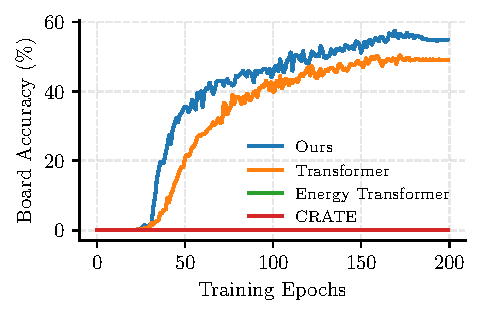
\includegraphics[width=\linewidth]{figures/sudoku_training_dynamics.pdf} %width=\linewidth
    % \vskip -.1in
    \caption{Sudoku training dynamics.}
    \label{fig:sudoku training}
  \end{subfigure}
  \hfill % Adds horizontal space between subfigures
  \begin{subfigure}[t]{0.49\textwidth}
    \centering
    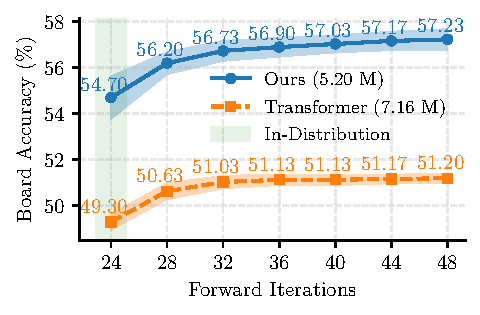
\includegraphics[width=\linewidth]{figures/sudoku_extropolation.pdf}
    % \vskip -.1in
    \caption{Sudoku test-time extrapolation.}
    \label{fig:test-time extrapolation}
  \end{subfigure}
  % \vskip -.1in
  \caption{\emph{Left}: Training dynamics of different approaches. Our model achieves a superior training curve, while Energy Transformer and \textsc{CRATE} both fail to make non-trivial predictions (\ie, flat curves). \emph{Right}: Test-time extrapolation w.r.t. forward iterations. Our model achieves better performance over five runs with fewer parameters, even when the iterations are beyond the training regime. }
  \label{fig:sudoku training dynamics test-time extrapolation}
\end{figure}